The ATLAS  detector's data acquisition system, illustrated in Figure \ref{fig:atlas_tdaq}, makes use of a multi-tiered trigger to reduce 
bandwidth from the LHC proton bunch crossing rate of 40 MHz
to the 1 kHz written to disk \cite{evolution1,evolution2}. The first tier (Level-1 or L1) \cite{l1}, implemented in real time with custom electronics, 
makes an early event selection to determine if any objects of interest are present and reduces the data flow to 
100 kHz. The second tier, referred to as the High Level Trigger (HLT) \cite{hlt}, is implemented on a commodity computing cluster running custom triggering software. The HLT uses information from the
hardware based L1 system to guide the retrieval of information from the Readout System (ROS) \cite{ros}. 

Jet, electromagnetic and tau clusters, missing transverse momentum ($E_{\mathrm{T}}^{\mathrm{miss}}$), $\sum E_{\mathrm{T}}$, 
jet $E_{\mathrm{T}}$, and muon candidate information from L1 determine detector Regions of Interest (RoIs) that seed HLT processing. These RoIs are provided to the HLT by a custom VMEbus based system, referred to as the Region of Interest Builder (RoIB) \cite{vme_roib}.
The RoIB collects data from L1 
trigger sources and assembles the data fragments into a complete record of L1 RoIs. These RoIs are made available to the HLT to initiate event processing. In order to improve maintainability and scalability, and to minimize the amount of custom hardware needing to be supported, 
the RoIB was implemented using commodity server hardware and an interface technology deployed 
within the ATLAS Trigger and Data Acquisition (TDAQ) system. The approach of implementing the RoIB functionality in software has been investigated in the past 
and the conclusion at that time was that a software based approach is possible but requires a card with a higher readout rate \cite{swroib_past}. 
Since data readout cards operating at high rates became available and the capabilities of computers have improved with the increase 
in CPU clock speed and number of cores, it became possible to implement the RoIB functionality using a PC based approach. 
The PC based RoIB must duplicate the functionality of the VMEbus based RoIB which means that the PC based solution must receive and assemble the
individual L1 fragments, and pass them as a single L1 result to the HLT. Modern computers have multicore CPU architectures 
with the possibility of running multi-threaded application, a feature which is being fully exploited in the RoIB software to achieve 
the desired performance of 100 kHz over 12 input links for fragment sizes of 400 bytes.  
This chapter describes the work of the author in evolving the RoIB from the VMEbus based system to the PC based system and gives details on the hardware, 
firmware, and software designs used to achieve the full RoIB functionality. 



\begin{figure}[tbp] % figures (and tables) should go top or bottom of
                    % the page where they are first cited or in
                    % subsequent pages
\centering
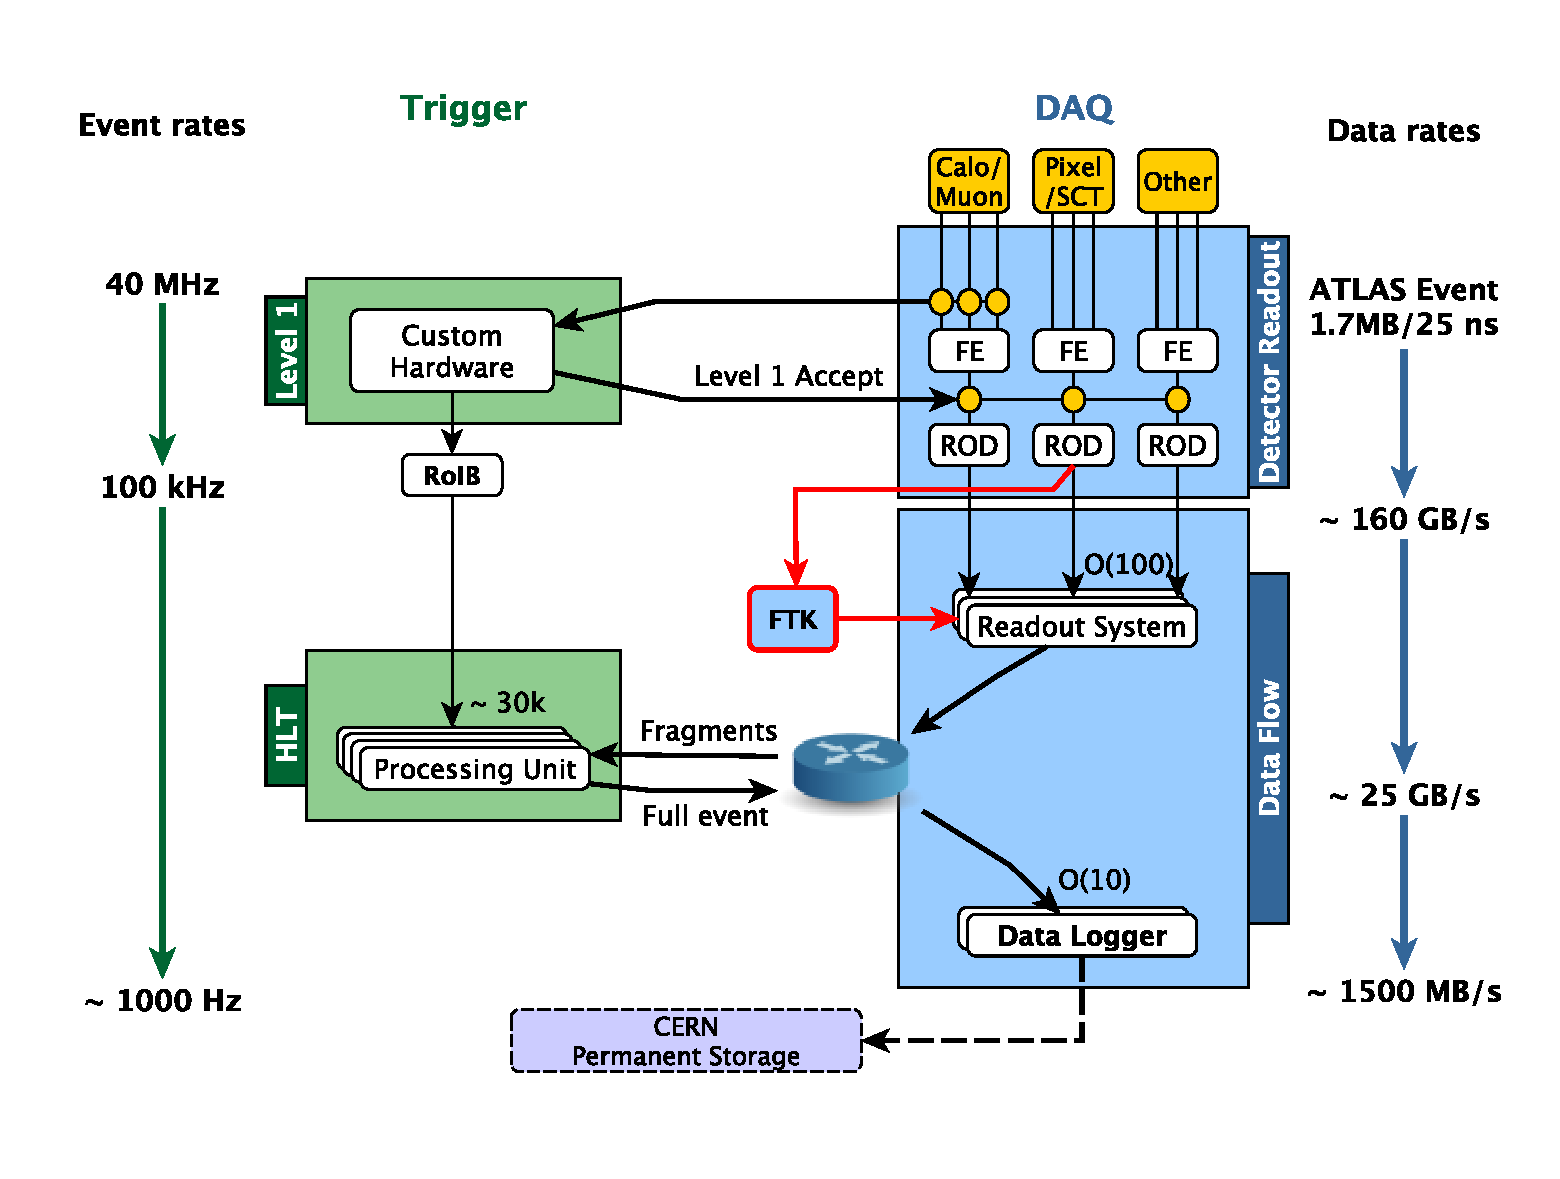
\includegraphics[width=.9\textwidth]{tdaqFullNew2015}
\caption{ATLAS TDAQ Architecture.}
\label{fig:atlas_tdaq}
\end{figure}



